\documentclass[12pt]{article}
\usepackage[colorlinks=true,bookmarks=false,citecolor=blue,urlcolor=blue]{hyperref}
\usepackage{listings}
\usepackage[margin=1in]{geometry}
\usepackage[style=authoryear]{biblatex}
\usepackage{setspace}
\usepackage{fancyvrb}
\usepackage{graphicx}

\onehalfspacing

\title{Chess}
\author{Gustavo Paz}

\begin{document}

\maketitle
\section{Introduction}
I, Gustavo A. Paz, created a network-enabled Chess game system that can be played 
through web browsers, securely. Users are able to create accounts, create 
and join Chess games to play against others, and search for players 
to see their game history and win/loss statistics. 
\maketitle
\section{Design Architecture}
I broke down the game system into 5 different components. The first was the front-end 
which was developed with Angular. Next are the two back-end webapp/services/endpoints the front-end
communicates with, IAM and Delegate, both developed with NodeJs. Next are the two database systems
the services communicate with to store game states and user authentication information, MongoDB 
and PostGreSQL.
\subsection{Front-end Architecture}
The front-end was developed with Angular. The front-end was broken down to views, models, and services.

\subsubsection{Models}
I will start by breaking down the models. Models are considered as plain old objects with a constructor 
and fields. The first one is the game model, it keeps track of the minimum information to display the game 
state to the users. Things like the history of moves, the chess board state, the player who's turn it is 
and so on. Next are the game-row and game-column models. They keep track of the chess board, which piece 
is in which place. Then the game-history model. This contains the move that users have made for a single 
game. Then we have the profile mode. This contains the win/loss statistics for a user and their game history. 
The user model maintains the relevant account session information of the user, such as user-id, username, role, and 
session token. The validation model is used to determine if validations were returned properly from the back-end services.

\subsubsection{Guard Models}
Thes are Angular guards that contain logic that should be executed before/after webpages in the application and can 
be used to re-route traffic.

The exit-history guard ensures the history object in the session storage is removed. The exit-profile guard ensures 
the profile object is removed from the session storage once the webpage using the guard is left from. The game 
guard is used to determine if a game object is in the session, then the only webpage that should be visible is the 
game state webpage. The history guard does not let the webpage from being visited if the history object is not 
set in the session storage. The linkguard is used for every webpage except the login to determine if the webpage is 
visible - only true when signed-in. The profile guard only allows access if a profile value is set in the session.


\subsubsection{Services}
The services are objects in the Angular app that send requests to the back-end services (IAM, Delegate) on behalf of 
the Angular app. There are two, the iam service and the delegate service. 

The iam service only communicates with the IAM back-end service to authenticate and create users. The method 
createAccount(username: string, password: string) sends requests to IAM to create accounts and sets the user once successful. 
On failure, the user is not created nor signed in. Next is login(username: string, password: string) which sends requests to 
authenticate users and sign them in - setting the user object in the session. There is also a helper method logout() which 
clears all the session information of the user signed in.

The delegate service only communicates with the Delegate back-end service to load and maintain game related information. 
The loadGameIfExists(user: User) sends a request to the back-end to load the last game the user was in to allow the user to rejoin. 
getGameState(gameId: string, token: string, userId: number) is used to load the latest game state of a game.
createGameState(token: string, userId: number, username: string) is used to create a new game with the user making the request 
as the player with the white Chess pieces. submitMove(fromColumnId: string, fromRowId: number, toColumnId: string, toRowId: number, 
gameId: string, token: string, userId: number, username: string) sends the move being made by the user for a specific game to the back-end service. 
getAllGames(userId: number, token: string) loads the 10 oldest games waiting for players to join. 
joinGame(gameId: string, userId: number, token: string, username: string, complete: () =\> void) makes a request to the back-end to 
set the second player of a game as the user making the request - upon a successful request the complete() method is called. 
quitGame(gameId: string, userId: number, token: string) sends a request to mark the game as a loss for the player sending the 
request - upon successful update the game is completed and the other player is marked as the winner. 
getProfile(userId: number, token: string, username: string, complete: () =\> void, failed: () =\> void) makes a request to load the profile 
for the username parameter - on sucess the complete method is called, on failure the failed method is called.

\subsubsection{Views}
The views the users interact with are the createaccount, find-game, find-user, game-state, history, login,
and profile.

The createaccount view allows users to create an account to play Chess games. It has an input field for the 
username and password. Once users enter values and click the create account button, the iam service is used 
to make a request to the IAM webapp to determine if the username is valid - ie: no other user has it - and returns a 
user with a session token on successful account creation.

The find-game view allows users to look for and join the 10 oldest games waiting for users to join. It also provides a link to 
allows users to join their last game if the game has not been timed out. This page uses DelegateService.joinGame() to join a game listed if 
anothe user has not joined; it also uses DelegateService.getAllGames() to load the 10 oldest games.

The find-user view provides a text-field for users to search for other users to then see their profiles. This page uses DelegateService.getProfile() 
to find and return profiles of valid usernames, if an invalid username is submitted a profile is not displayed.

The game-state view provides an interface for users to view the game state and move piece in the user's current game. This page 
uses DelegateService.getGameState() to load the game state, DelegateService.submitMove() to submit valid moves, and DelegateService.quitGame() 
to quit games.

The history view provides users the ability to see the history on a specific game - who moved what and where from/to - 
the object returned by DelegateService.getProfile() contains the game history information.

The login view allows users to login to their account - IamService.login() is used to log users in.

The profile view displays the game history of users and they're win/loss statistics - the DelegateService.getProfile method 
is used to load the related information.

\subsection{Database Architecture}
The two databases I used for the project are MongoDB and PostGreSQL. I used PostGreSQL specifically for the IAM service 
because authentication information never changes and relation databases provide good storage for data that does not constantly 
- like the game states. Given the user account information does not change after creation, this type of database was ideal for 
the IAM service. I then used MongoDB to store game state information. Unlike relational databases NoSQL provides great 
performance for constant writes and reads which is why I used it to store the game states since they're constantly being updated 
while games are being played.


\subsubsection{PostGreSQL Tables}
There are 6 tables used to store and manage user identity information. The first is the permission table, which stores all 
the permissions roles are given. The role permission table assigns permissions to roles. The role table keeps track of the different 
roles for the application, for this application there is one, 'Hikaru'. Next is the user role table which assigns users to roles. 
Next we have the  user table which stores the user information such as the username and creation date. Finally we have the user sec 
table which stores the passwords for accounts and the salts used to generate the passwords. As in the diagram below, there are 
foreign key, not-null constraints, and unique constraints to ensure the data is consistent.

\begin{figure}[h!]
    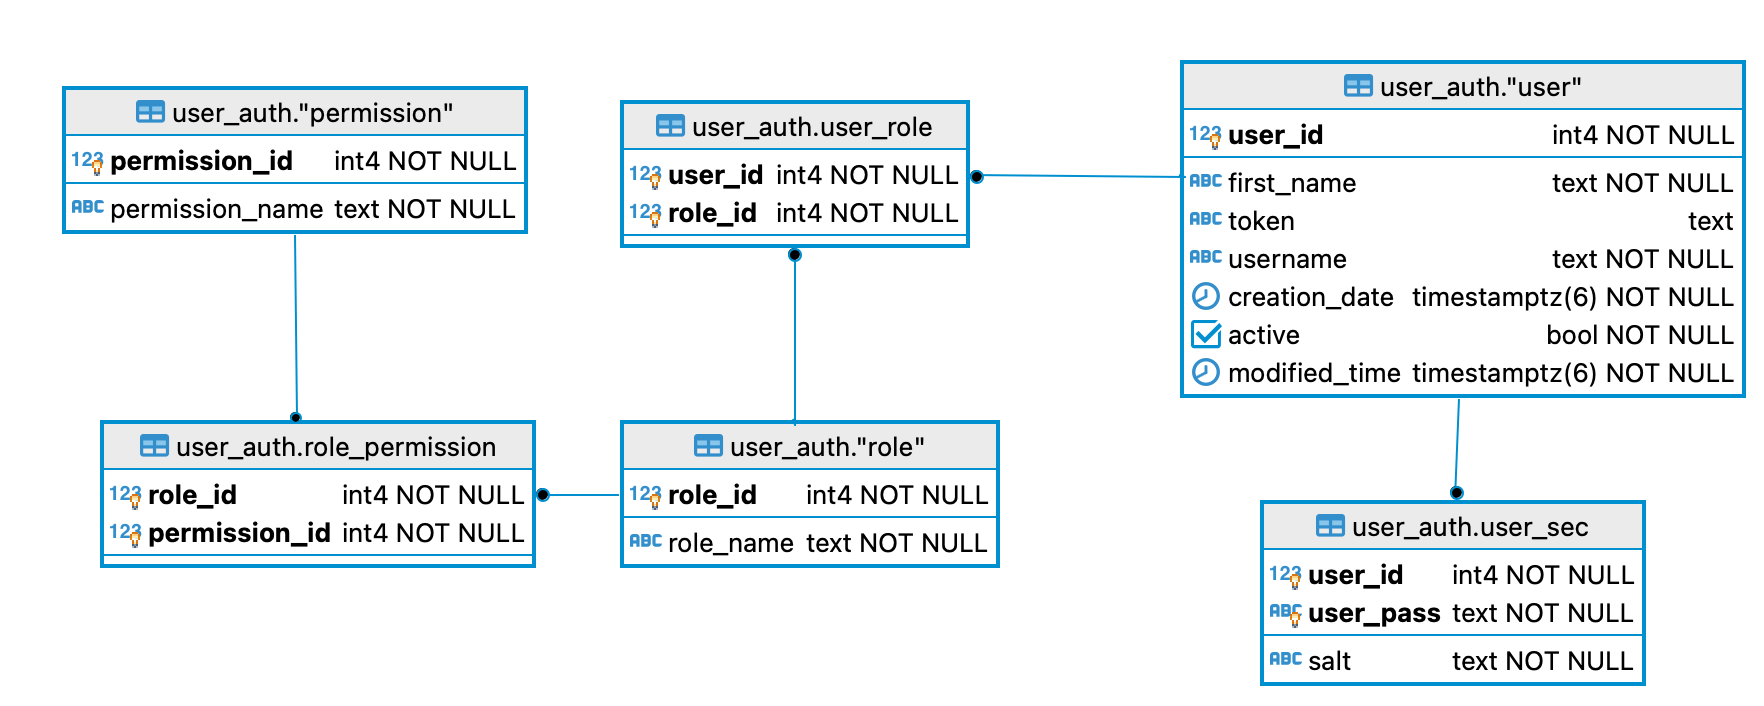
\includegraphics[width=\linewidth]{postgres.png}
    \caption{ER Diagram}
\end{figure}

\subsubsection{MongoDB Structure}
The database has only one collection which is 'chess'. Entries in this collection keep track of games. The id column is for the game id. It maintains usernames and ids along with the winner's username and id. There is a state column which maintains the state of the board and a fenState column which is used in conjunction with a board validator to ensure the game state and moves are valid. The history column maintains the moves of each player while maintaining the order of said moves - the tracebility of the game. 
The state field maintains the game as a set of rows with columns with their column id and the piece at each column - directly mapping to the board state users see on the front-end.

\subsection{Back-end Architecture}
The back-end consists of two different NodeJs servers. One is the IAM service, which handles user account identity management. Then is the Delegate service, which handles the game information.

\subsubsection{IAM Service}
This service is developed in NodeJs and communicates with with the PostGreSQL database.

\subsubsection{IAM Service Configuration}
The service listens on the 8000 port and uses the express library and cors library to receive requests from the front-end. Express provides a way to easily add POST/GET endpoints to the service. For requests received, I've added the express.json() middleware that only parses json and only looks at requests where the Content-Type header matches the type option - given I only send json type data to this service this seemed fit. Along with this I added express.urlencoded() to the service which parses urlencoded bodies for POST requests this service receives. The cors library provides is a middleware that enables CORS for the service so only GET and POST requests coming from the front-end, specifically 'https://localhost:4200', are allowed. Furthermore the service sets its key, cert, and certificate authority which are used to authenticate SSL/TLS connections from the front-end.

The database connection is also configured and set using node-postgres which is built on top of the built-in TLS library. So when we provide the service certificate, key, and db certificate, the connection is assured to be secure. This library also allows us to set timeouts on query and statement processing to lessen the possibility of hanging requests.


\subsubsection{IAM Service Endpoints}

First we have the POST endpoint, '/iapi/createaccount'. This endpoint handles the request to create new accounts. It first validates the parameters are not null and valid string values. It expects username and password as the parameters to the request. A salt is then generated with the bcrypt library function genSaltSync() which generates a salt to be used to hash the password. Next a hash of the password is created using the bcrypt's hashSync(password, salt) function. Next it opens a connection to the database and begins a transaction. Once the transaction has started the create user SQL is executed to insert a new user with the username parameter which will return the user id for the new user - the database has a sequence and a unique constraint on the id and username columns to ensure this is no conflicting data. Once the user id is returned the query to insert user seq information, such as the hashed password, user id, and the salt used to generate the hash password are stored so when users try to sign in. Next the role is assigned to the user executing the assgin role query which assigns the 'Hikaru' role. Then a session token is generated using the jsonwebtoken library. The values set in the token are the user id, while only making it valid for 24 hours, and providing the web application certificate to sign it. Lastly the transaction is committed to the database and the new user is returned to the front-end with the token, user id, username, and role. In the event the transaction fails for some reason, the catch clause will rollback any changes that occurred during the transaction.

Second we have the POST endpoint, '/iapi/authenticate'. This endpoint handles all requests to authenticate users trying to sign in the application. Similar to the createaccount endpoint it first validates the parameters are not null and valid string values. It expects username and password as the parameters to the request. Next it opens a connection to the database and begins a transaction. 
\subsubsection{}

\maketitle
\section{Installation Instructions}

\maketitle
\section{Operation Instructions}

\maketitle
\section{Game Rules}

\maketitle
\section{Why is it secure?}

\end{document}
